\section{System Identification of a Soft Robot}
\label{sec:experiment}

To demonstrate and evaluate the performance of the method outlined in Section \ref{sec:theory}, we applied it to a continuously deformable soft robot arm and compared the resulting model to those generated by other nonlinear system identification techniques.
In the following, we explain in detail the used robotic hardware, experimental setup, measurement procedure, and the data processing involved in the system identification process, as well as the process by which performance was evaluated and compared across models.
% \David{In the following, we explain in detail the used robotic hardware, experimental setup, measurement proces, ...}This section describes the composition of the robot and recount the setup, measurement, and data pre-proccessing involved in the system identification process.


\subsection{Hardware Description}

The soft robot used in this experiment consisted of three pneumatically driven McKibben actuators (also known as Pneumatic Artificial Muscles or PAMs) adhered together by latex rubber and connected to a common base mount on one end and to an end effector on the other (see Fig. \ref{fig:flaccy}).
During the trials, the pressure inside each actuator was varied using a pneumatic pressure regulator (Enfield TR-010-g10-s), and the displacement and velocity of the end effector was measured at $60 \text{Hz}$ using a commercial motion capture system (Phase Space Impulse X2E).

%% state space representation of model
For this robot, it is our primary interest to control the motion of the end effector.
% \David{Try to use more declarative language.  We have discussed this in the past.  Other people do a lot of different things (and might disagree in your notion of primary interest), but you can simply say what your interest is: ``Our declared control goal for this setup is to dynamically control the kinematic motion of ...} With robotic manipulators, it is often of primary interest to dynamically control the motion of the end effector.
% \David{To this end, we chose...} 
Hence, we chose a state representation of the system which is capable of describing the dynamics of the end effector as an ordinary differential equation, namely the position and velocity of the end effector with respect to a global coordinate frame, as shown in Fig. \ref{fig:flaccy}
% Hence, we chose to represent the state of our soft robot as the position and velocity of the end effector with respect to a global coordinate frame, as shown in Fig. \ref{fig:flaccy}
\begin{align}
    \vec{x} &= \mtx{ x_1 & x_2 & x_3 & \dot{x_1} & \dot{x_2} & \dot{x_3} }^T
    \label{eq:state}
\end{align}

\subsection{Randomized Control Input}

To generate a representative sampling of the system's behavior over its entire operation range, a randomized input was applied.
The control input into the system $\uv$ was a set of three $0-10 \text{V}$ signals into the pressure regulators corresponding to actuator pressures of $\approx 0-140 \text{ kPa}$
\aln{
    \uv (t) &= \mtx{ u_1 (t) & u_2 (t) & u_3 (t) }^T,   && u_i \in [0,10]
}
Before each trial, a $3 \times 1000$ table $\Upsilon$ of uniformly distributed random numbers between zero and ten was generated to be used as an input lookup table.
Each control input was smoothly varied between elements in consecutive columns of the table over a transition period $T_u$, with a time offset of $T_u / 3$ between each of the three control signals
\aln{
    u_i (t) &= \frac{(\Upsilon_{i,k+1} - \Upsilon_{i,k})}{T_u} \left( t + \frac{(i-1) T_u}{3} \right) + \Upsilon_{i,k}
    \label{eq:input}
}
where $k = \text{floor}\left( {t} / {T_u} \right)$ is the current index into the lookup table at time $t$. 
% (see Fig. \ref{fig:randInput}).

%% Figure: Randomized Inputs
% \begin{figure}
%     \centering
%     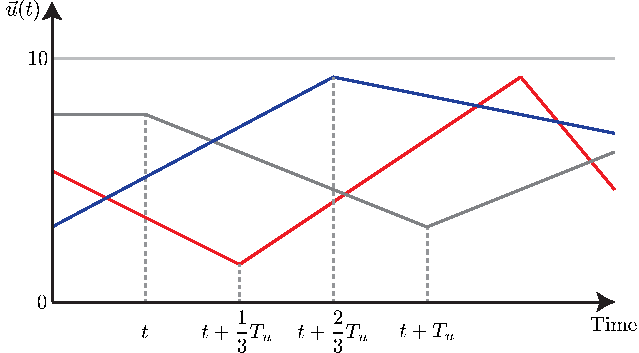
\includegraphics[width=\linewidth]{figures/randInput3dim.pdf}
%     \caption{Caption: Randomized control inputs \David{I would add the dotted line at t+4/3T.}}
%     \label{fig:randInput}
% \end{figure}


\subsection{Data Collection}

% %% TABLE: Trial parameters
% \begin{table}[h]
%     \centering
%     \caption{Data Collection Parameters}
%     \begin{tabular}{|c||c|c|}
%         \hline
%          & $\bm{T_u}$ \textbf{(s)} & \textbf{Length (min)} \\
%         \hline
%          Trial 1 & 3 & 40:06 \\
%          Trial 2 & 3.5 & 31:26 \\
%          Trial 3 & 4 & 8:16 \\
%          Trial 4 & 5 & 26:09 \\
%          Trial 5 & 5 & 28:38 \\
%          Trial 6 & 8 & 31:35 \\
%         \hline
%     \end{tabular}
%     \label{tab:trialParams}
% \end{table}

%% TABLE: Trial parameters (ONLY IF TWO ROBOTS ARE USED)
% \begin{table}[h]
%     \centering
%     \caption{Data Collection Parameters}
%     \begin{tabular}{|c||c|c||c|c|}
%         \hline
%         & \multicolumn{2}{c|}{Robot A} & \multicolumn{2}{c|}{Robot B} \\
%         \hline
%          & $\bm{T_u}$ \textbf{(s)} & \textbf{Length (min)} & $\bm{T_u}$ \textbf{(s)} & \textbf{Length (min)} \\
%         \hline
%          Trial 1 & 3   & 40:06 & 2   & \\
%          Trial 2 & 3.5 & 31:26 & 3   & \\
%          Trial 3 & 4   & 8:16  & 3.5 & \\
%          Trial 4 & 5   & 26:09 & 4   & \\
%          Trial 5 & 5   & 28:38 & 5   & \\
%          Trial 6 & 8   & 31:35 & 6   & \\
%         \hline
%     \end{tabular}
%     \label{tab:trialParams2}
% \end{table}

Data collection proceeded in 4 trials, each lasting between 8 and 40 minutes with an input transition period $T_u$ between 3 and 8 seconds. 
% The specific testing parameters for each trial can be found in Table \ref{tab:trialParams}.
After collecting data, raw position and velocity measurements were put through a moving average filter with window size of $1$s to reduce noise, then sampled uniformly with a period $T_s = 0.02 \text{s}$.
Sampled velocity measurements were put through a second moving average filter with window size of $1$s, due to the higher noise content of the velocity signal.
%% Partitioning of trail data into training and validation sets
The time-series data from each trial was partitioned into training and validation sets. 
Three 10 second validation sets were extracted from each trial and the remainder of the trial data was used for training.

%% FIGURE: Showing what flaccy looks like
\begin{figure}
    \centering
    \vspace{10pt}
    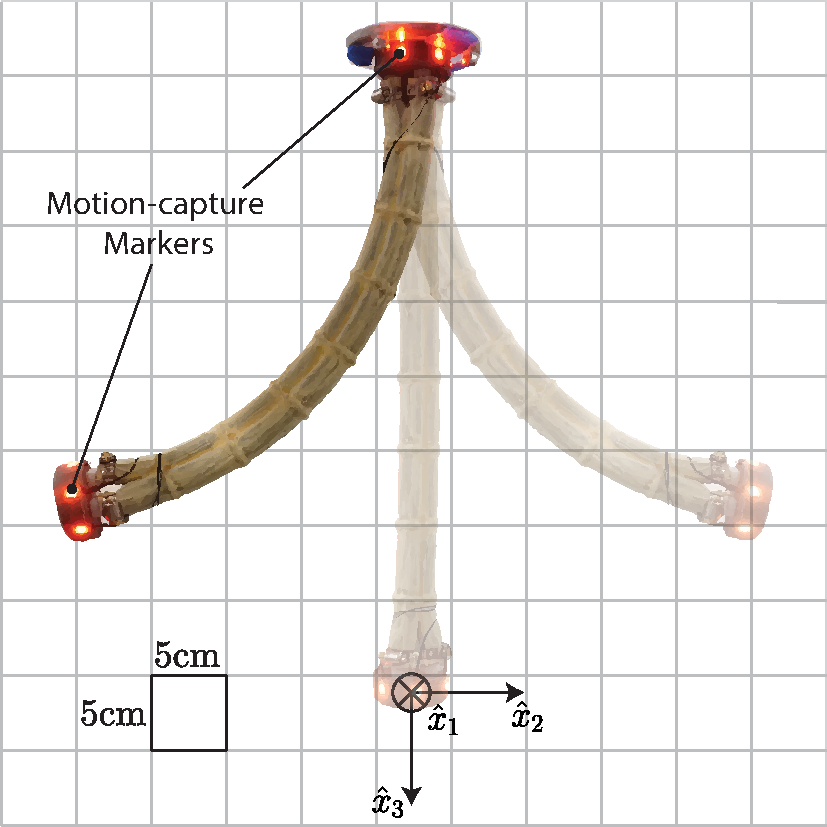
\includegraphics[width=0.95\linewidth]{figures/flaccyDiagram_bothways_v4.pdf}
    \caption{System identification was performed on a soft robot consisting of three PAMs adhered together. 
        Active motion capture markers on the base and end effector enabled tracking of the position and velocity of the end effector relative to the fixed global coordinate frame marked by unit vectors $\hat{x}_1,\hat{x}_2,\hat{x}_3$. The robot's range of motion given control inputs defined in \eqref{eq:input} is depicted.}
    \label{fig:flaccy}
\end{figure}


%% Model Comparison
\subsection{Model Comparison}
\label{sec:modelcomparison}

%% Performance was evaluated by comparing simulations to real measurements
We generated a state space model from the technique described in section \ref{sec:theory} using a monomial basis of maximum degree $w=3$.
We then evaluated its accuracy by comparing model simulations to validation data (Fig. \ref{fig:koopmanSim}).
Goodness of fit for the trajectory of a state $y$ was calculated using the normalized root-mean-square error (NRMSE), defined:
%% Normalized Root Mean-Square Error
\aln{
    \text{RMSE} &= \sqrt{ \frac{\sum_{k=1}^{N_\text{total}} \left( y_k - \hat{y}_k \right)^2}{N_\text{total}} } \\
    \text{NRMSE} &= \left( \frac{\text{RMSE}}{y_\text{max} - y_\text{min}} \right) \cdot 100 \%
    % 1 - \frac{ \| y - \hat{y}  \| }{ \| y - \text{mean}(y) \| }
}
where $\hat{y}$ is the simulated value of the state, $N_\text{total}$ is the total number of points, and $y_{\text{min/max}}$ are the measured minimum/maximum values of the state observed over all trials.

%% For comparison, other sysid methods were also used on the same set of data
The performance of our model was benchmarked against a linear state space, nonlinear Hammerstein-Wiener, nonlinear auto-regressive with exogenous inputs (NLARX), and a neural network model.
All models were trained and evaluated on the same training and evaluation data and generated using either the Matlab System Identification Toolbox or Neural Network Toolbox \cite{MATLAB:2017}.
The state space model was generated using the subspace method \cite[Chapter 7]{ljung1987system} and specified to be 6 dimensional, i.e. the same dimension as the state defined in \ref{eq:state}.
The neural network model was trained using the Levenberg-Marquardt backpropogation algorithm and sigmoid activation functions.
It was trained several times using combinations of 10-30 hidden neurons and 1-10 delays.
Only the results for the best of these models, corresponding to 10 hidden neurons and 10 delays, is displayed in Fig. \ref{fig:comparison} and Table \ref{tab:RMSE}.